\documentclass{article}
\usepackage{hyperref}
\usepackage{enumitem}
\usepackage[margin=1in]{geometry}
\usepackage{graphicx}
\usepackage{fancyhdr}
\usepackage{minted}
\usepackage{float}
\graphicspath{{Images/}}

\hypersetup{
	colorlinks=true, %set true if you want colored links
	linkcolor=black,  %choose some color if you want links to stand out
}

\pagestyle{fancy}
\rfoot{
\includegraphics[scale=0.4]{IITlogo}}

\title{ECE 100 Laboratory 01 Instructions }
\author{Illinois Institute of Technology ECE Department}
\date{Last Modified: \today}



\begin{document}
	\maketitle
	
	\paragraph{Lab Objective} Complete the OSOYOO Robot Kit assembly and install and run provided software in Arduino IDE. 
	
	\section{Hardware Installation}
	
	\paragraph{Introduction} Below are the instructions on how to properly assemble the OSOYOO Robot. Please follow the instructions as listed to complete the build by the end of the Lab section. The instructions provided below are adapted from the OSOYOO provided instructions for your ease of use. If you wish to have additional support in the build process, navigate to the following link for a video tutorial.
	
	\vspace{1em}
	
	\href{https://osoyoo.com/2020/05/12/osoyoo-v2-1-robot-car-kit-lesson-1-basic-robot-car/}{Robot Build Instructions Page}
	
	
	\begin{enumerate}
		\item Remove the protective film on the upper and lower car chassis. Each car chassis has one protective film. The protective film is covering the print text on the top of each 
		chassis layer. 
		
		\begin{figure}[H]
			\centering
			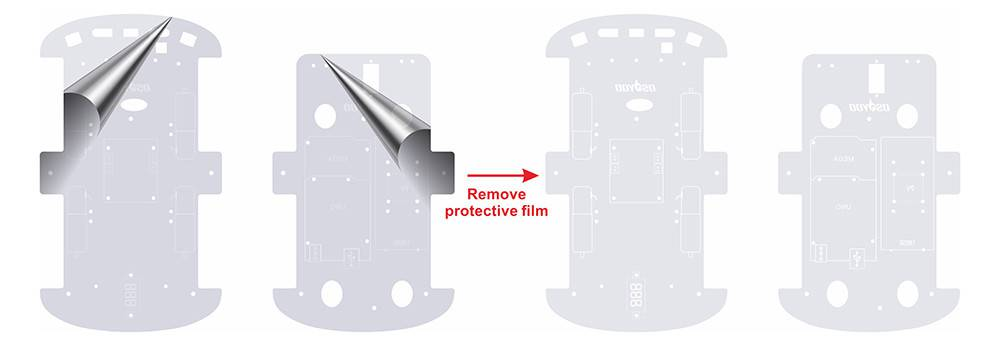
\includegraphics[width=0.7\linewidth]{image1}
			\label{fig:image1}
		\end{figure}
		
		
		\item Install the motor holders on each of the four motors. The direction in which these holders are mounted is important to note as it corresponds to the chassis mounting. All motors should have the motor mounts attached on the side to which the wires are attached. As you will see in instruction step 3, the four motors will be attached to the chassis, with two motors mirroring each other. Ensure that the mounts are installed so that the motor mount holes align with the holes on the larger base chassis. For aesthetic purposes, ensure that the head of the bolts to attach the motor holder are on the side that does not have the wires (opposite of the motor holder). The image below shows the correct orientation of the motor mounts.
		
		\begin{figure}[H]
			\centering
			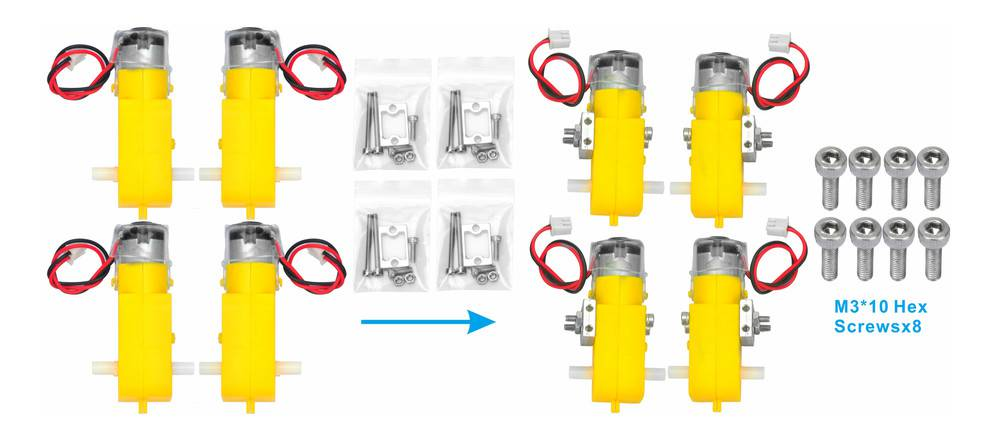
\includegraphics[width=0.7\linewidth]{image2}
			\label{fig:image2}
		\end{figure}
		
		\item Fix the four motors on the large base car chassis using the M3*10 hex screws and the provided hex screwdriver. You can find the two screws per motor in the packaging of the motor holder. See the image below for proper orientation.
		
		\begin{figure}[H]
			\centering
			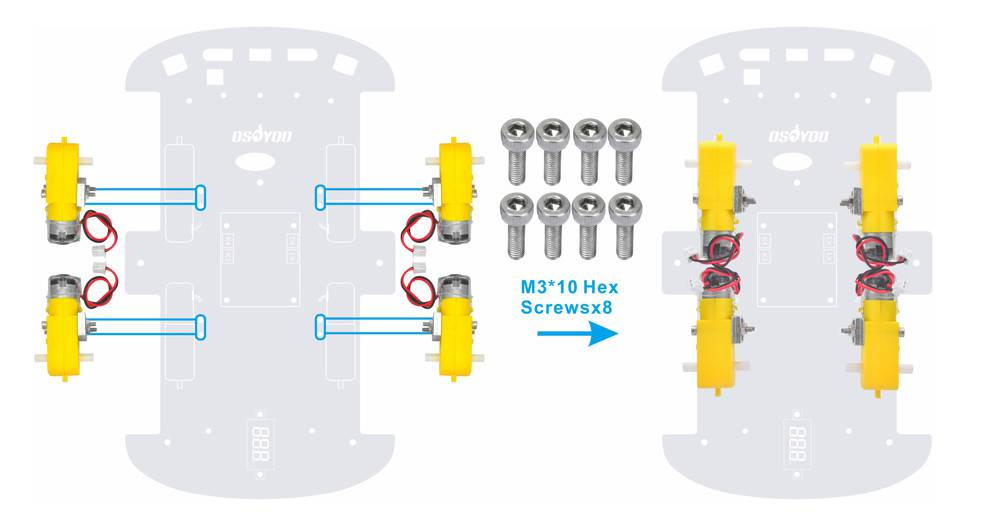
\includegraphics[width=0.7\linewidth]{image3}
			\label{fig:image3}
		\end{figure}
		
		\item Install OSOYOO MODEL X motor driver to the base chassis using 4 M3 plastic screws, plastic pillars, and plastic nuts. The heat sync on the motor driver (a large black metal piece with multiple fringed panels) should be closest to the printed image on the board of 3 seven-segment displays (where the voltage meter will be mounted).
		
		\begin{figure}[H]
			\centering
			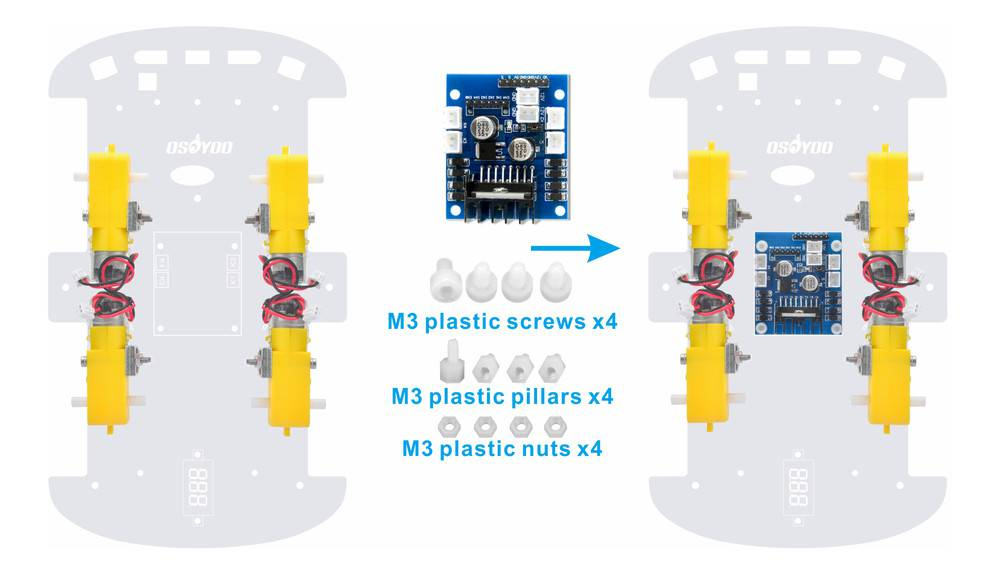
\includegraphics[width=0.7\linewidth]{image4}
			\label{fig:image4}
		\end{figure}
		
		\item Install the voltage meter on base car chassis using 2 M3 plastic screws, plastic pillars, and plastic nuts. The three jumper cable pins should be oriented inwards towards the motor driver.
		
		\begin{figure}[H]
			\centering
			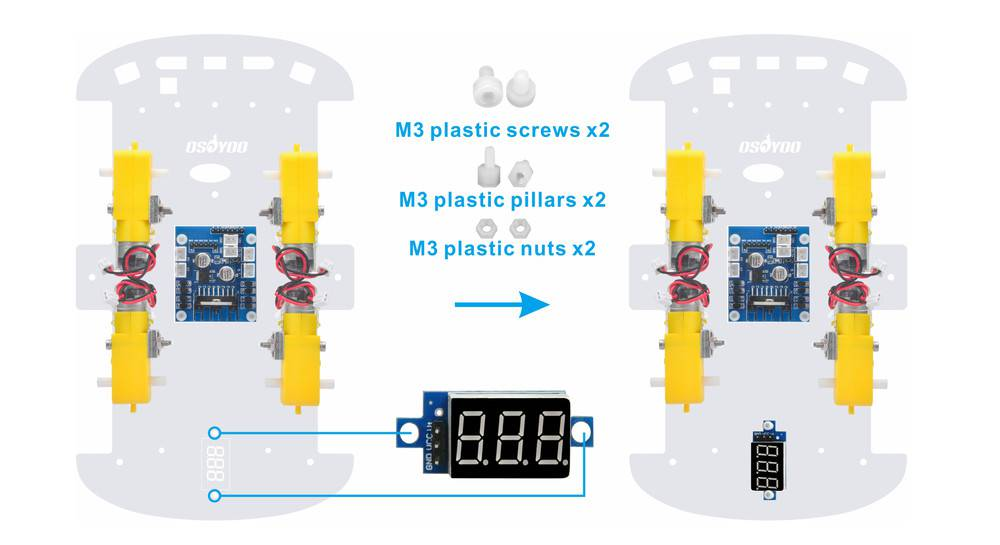
\includegraphics[width=0.7\linewidth]{image5}
			\label{fig:image5}
		\end{figure}
		
		\item Fix OSOYOO UNO R3 board (your Arduino!) to the upper car chassis using 4 M3 plastic screws, plastic pillars, and plastic nuts. The USB A/B connector should be facing the back of the car, opposite the OSOYOO logo on the chassis.
		
		\begin{figure}[H]
			\centering
			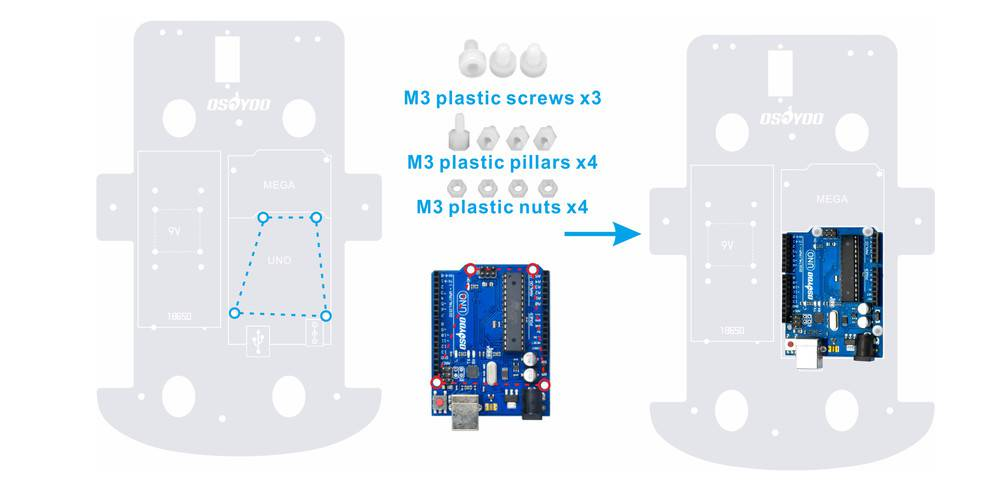
\includegraphics[width=0.7\linewidth]{image6}
			\label{fig:image6}
		\end{figure}
		
		\item Fix the 18650 Battery Box on the upper chassis using four M3x10 screws and M3 nuts. The wires from the box should be facing away from the OSOYOO logo.
		
		\begin{figure}[H]
			\centering
			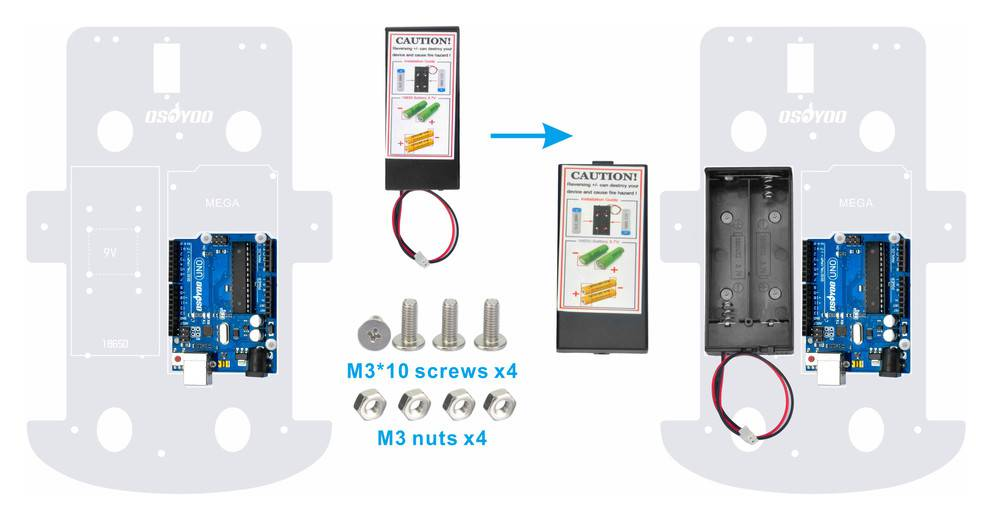
\includegraphics[width=0.7\linewidth]{image7}
			\label{fig:image7}
		\end{figure}
		
		\item Insert the OSOYOO Uart WIFI shield V1.3 onto the UNO board. The side of the board that has the tab with gold routing should be facing the back of the car opposite of the OSOYOO logo. Slide the pins of the WIFI shield into the corresponding pins on the UNO board.
		
		\begin{figure}[H]
			\centering
			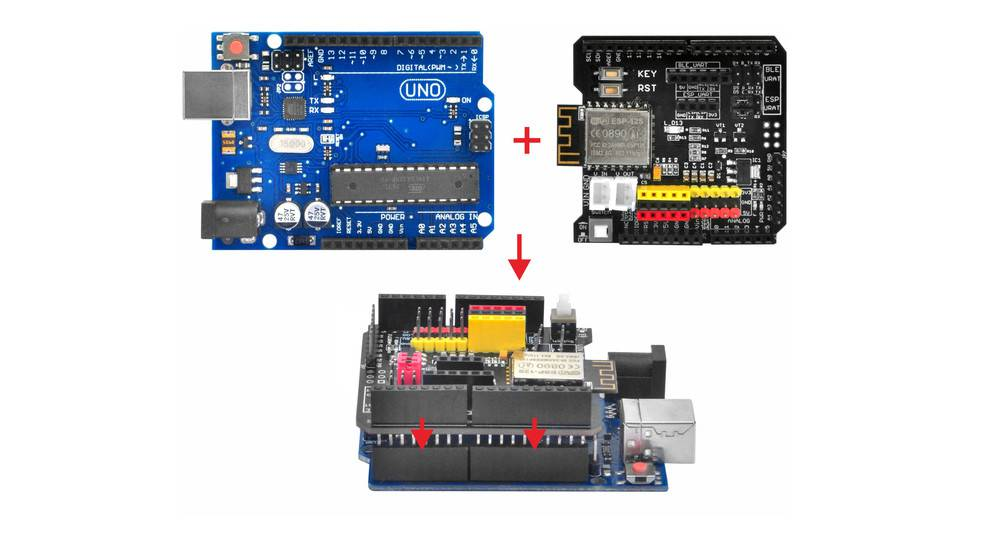
\includegraphics[width=0.7\linewidth]{image8}
			\label{fig:image8}
		\end{figure}
		
		\item Begin the wiring connections of the motors as shown. The cables from the motor will be mounted into the closest connection of the motor driver module.
		
		\begin{figure}[H]
			\centering
			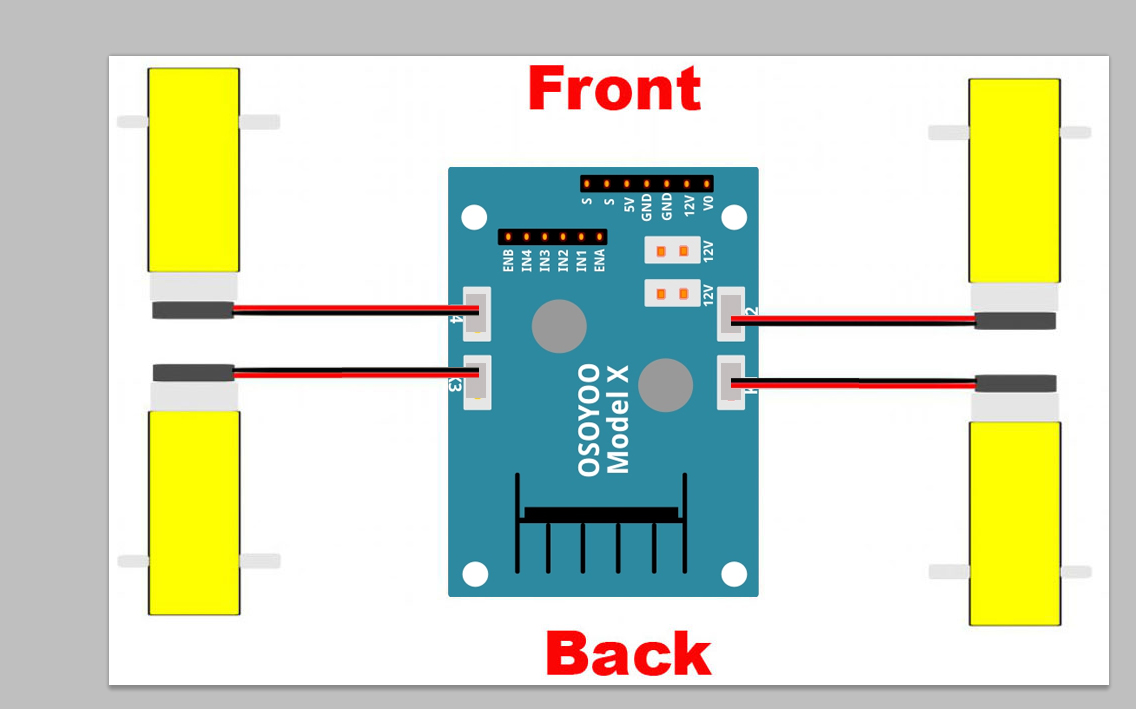
\includegraphics[width=0.7\linewidth]{image9}
			\label{fig:image9}
		\end{figure}
		
		\item Using the 3-pin female to female jumper wire that contains two red and one black wire, connect the voltage meter to the motor driver as shown in the image below.
		
		\begin{figure}[H]
			\centering
			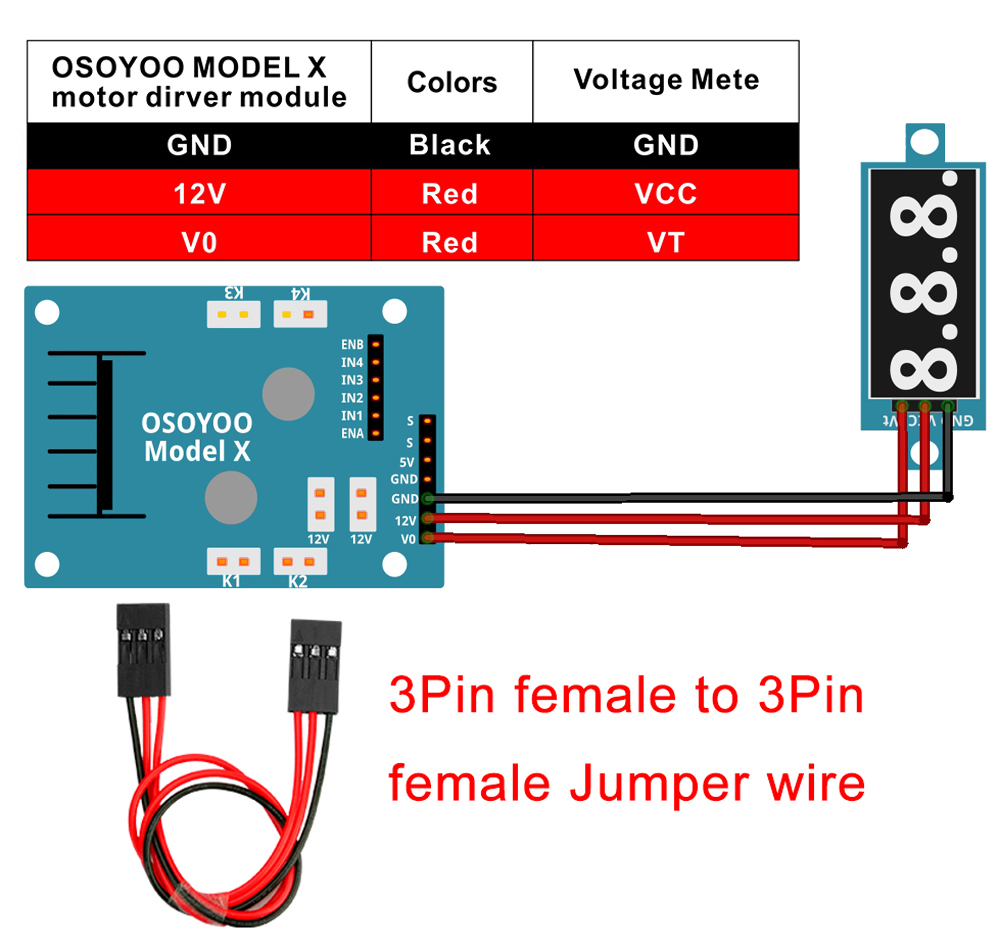
\includegraphics[width=0.7\linewidth]{image10}
			\label{fig:image10}
		\end{figure}
		
		\item Connect OSOYOO MODEL X motor driver module 6 control pins to OSOYOO Uart WiFi shield V1.3. Ports D6, D7, D8, D9, D11, D12 will be connected with 6pin male to 6pin female jumper wire (Contains red, white, yellow, green, purple, and black wires). Make sure to leave D10 unoccupied. When routing, you will be moving from the bottom chassis to the top chassis. Route the cables through the front right hole on the upper chassis, to the right of the OSOYOO logo.
		
		\begin{figure}[H]
			\centering
			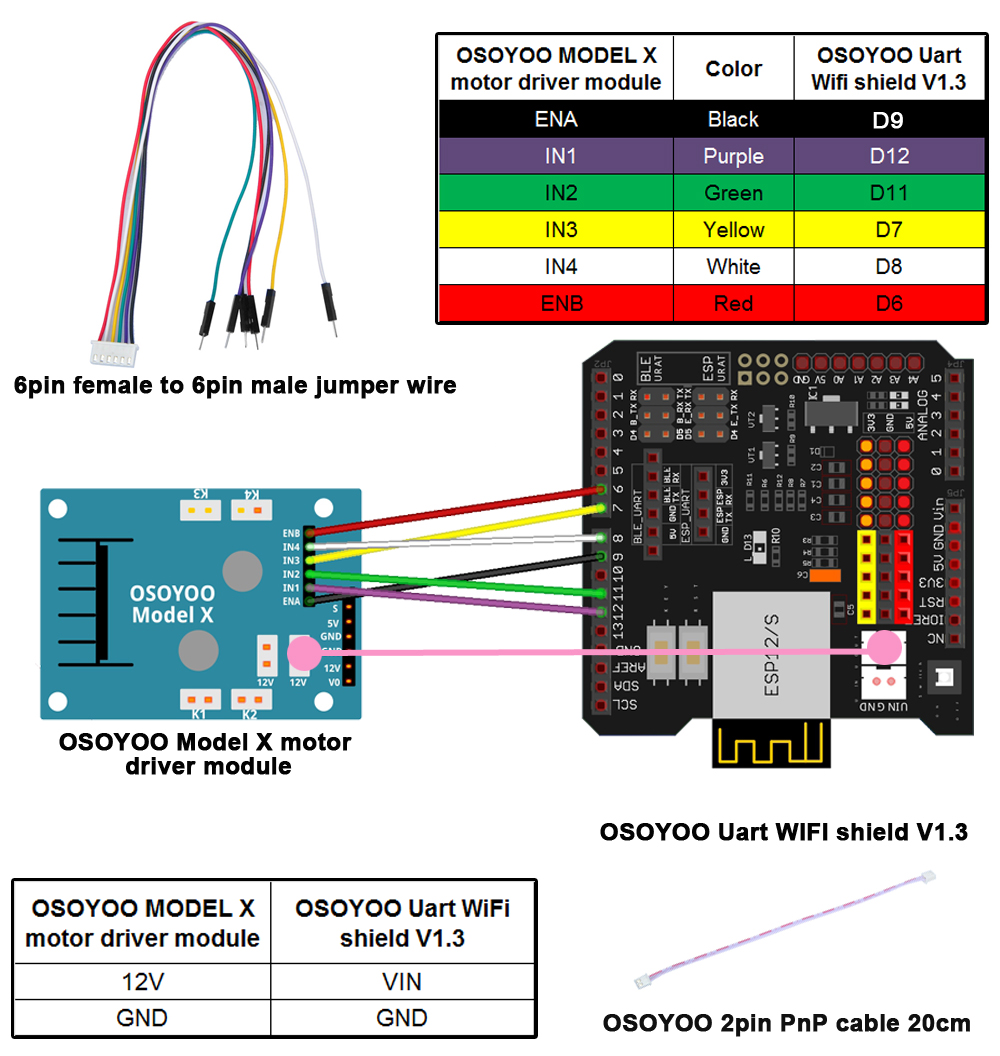
\includegraphics[width=0.7\linewidth]{image11}
			\label{fig:image11}
		\end{figure}
		
		\item Connect the 12V-GND socket to the VIN-GND socket with OSOYOO 2pin PnP cable 20cm as shown in the previous image. The cables will both be light purple, so use the orientation of the plastic connector to guide. Route the cable through the same hole in the chassis as in step 11. When installing and removing this cable (or any other that contains a plastic connector), ensure to pull from the plastic connector rather than the cables to prevent any damage. 
		
		
		
		\item Connect the cables from the battery box to the VIN-GND socket of the OSOYOO Uart Wifi Shield. Orientation can be seen in the image below.
		
		\begin{figure}[H]
			\centering
			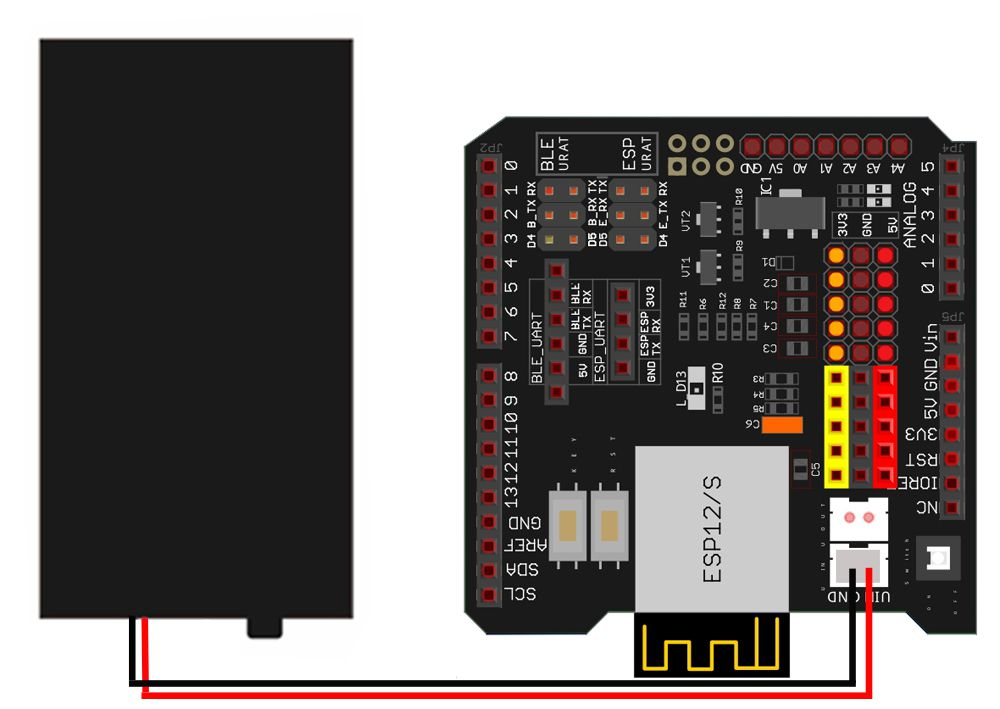
\includegraphics[width=0.7\linewidth]{image13}
			\label{fig:image13}
		\end{figure}
		
		\item Mount the upper and lower part of the chassis with five copper pillars and secure the pillars using two M3*10 hex screws for each pillar. The hex screw heads should sit flush on the top and base of the chassis. There are additional holes on the chassis base, so make sure to check with the image below to ensure the pillars are mounted correctly.
		
		\begin{figure}[H]
			\centering
			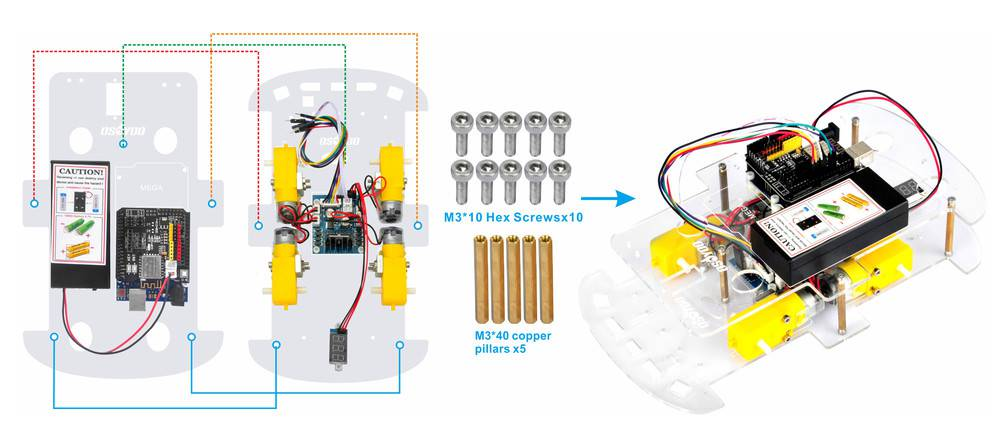
\includegraphics[width=0.7\linewidth]{image14}
			\label{fig:image14}
		\end{figure}
		
		\item Install the four wheels onto the shaft of the motor. Secure the wheels using the screws for the wheels provided in the kit.
		
		\begin{figure}[H]
			\centering
			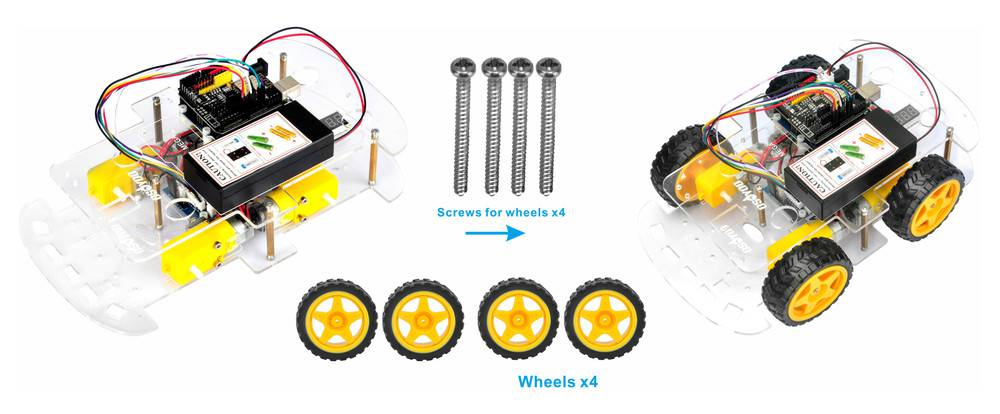
\includegraphics[width=0.7\linewidth]{image15}
			\label{fig:image15}
		\end{figure}
		
		\item \textbf{Congrats, your hardware installation is complete! Pick a name for your latest creation and head onto the software installation.}
		
	\end{enumerate}
	
	\section{Software Installation}
	
	\begin{enumerate}
		\item Install latest Arduino IDE (If you have Arduino IDE version after 1.1.16, please skip this step). Download Arduino IDE from \href{https://www.arduino.cc/en/Main/Software?setlang=en}{this link}, then install the software.
		
		\item Download Lesson One sample code from \href{https://osoyoo.com/driver/v2smartcar-lesson1.zip}{this link}, unzip the download zip file smartcar-lesson1.zip, you will see a folder called v2smartcar-lesson1.
		
		\item Connect Arduino UNO to PC with USB 2.0 A/B cable. Open Arduino IDE $\rightarrow$ click file $\rightarrow$ click Open $\rightarrow$ choose code \texttt{\textit{v2smartcar-lesson1.ino}} in smartcar-lesson1 folder.
		
		\begin{figure}[H]
			\centering
			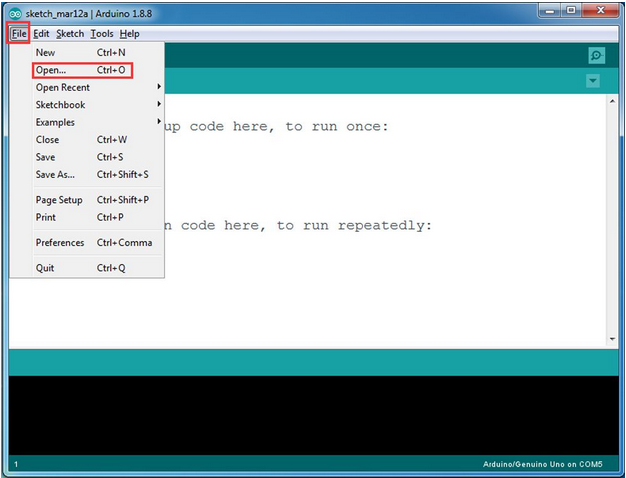
\includegraphics[width=0.7\linewidth]{Images/s1}
			\label{fig:s1}
		\end{figure}
		
		
		\item In the IDE, select the correct board for the project. Navigate to Tools, then “board. “ A side menu will appear with a variety of options. Select “Arduino Uno.” Regarding the port, it should default to the port in which the USB was plugged. If you are having trouble connecting to the board, go to your Device Manager on your PC, go to “Universal Serial Bus controllers,” and unplug the Arduino board. The port used will no longer appear on the list. Plug it back in to verify the correct port, and it should appear on the list once again.
		
		\begin{figure}[H]
			\centering
			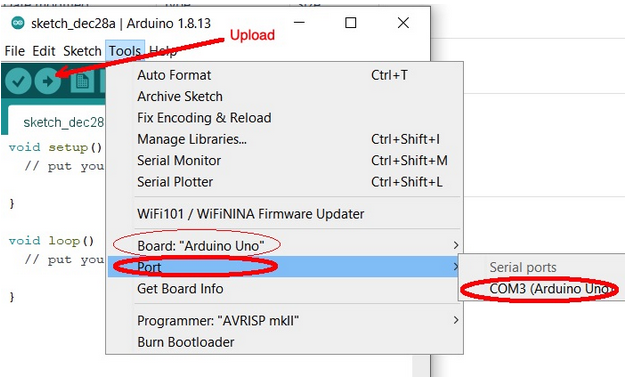
\includegraphics[width=0.7\linewidth]{Images/s2}
			\label{fig:s2}
		\end{figure}
		
		
		\item Upload the code to the board using the right arrow button as shown in the previous image. Once it is done uploading the code, the bottom right should display \texttt{\textit{Done Uploading}}.
		
	\end{enumerate}
	\textbf{Now you’re all prepped! Go to Final Testing to run your robot! }
	
	\section{Final Testing}
	
	\begin{enumerate}
		\item Disconnect the Arduino from the PC
		\item Install 18650 batteries into Battery Box. Please ensure that the polarity is correct, otherwise the system will likely be destroyed if turned on. 
		\item Place the car on the ground.
		\item Turn on the battery box connected to the WiFi Shield. 
		\item Press the white square button on the back right corner of the OSOYOO Uart WiFi Shield. 
		\item If all steps have been done correctly, the car will move forward for 2 seconds, backward for 2 seconds, left turn for 2 seconds, then right turn for 2 seconds.
		
	\end{enumerate}
	
\end{document}